%=============================================================================
% Drop-in Experiments section. Insert into template_revised.tex immediately
% AFTER the end of \subsection{General PSD Graph Kernels} (currently the last
% subsection of §3 Main Results, ending around line 786) and BEFORE the
% bibliography block (\bibliographystyle / \bibliography, around line 791).
% This makes Experiments §4, with the appendix-deferred Related Work
% remaining as it is.
%
% Required figure files (already in the repo):
%   experiments/outputs/exp2_density_sweep.png
%   experiments/outputs/exp3_smoothness_asymptotics.png
%
% Uses only macros and labels already defined in template_revised.tex; no new
% packages needed.
%=============================================================================

\section{Experiments}\label{sec:experiments}

We empirically substantiate two of the four quantitative claims of
\S\ref{sec:main-results}: the graph-feedback hardness $H_{\mathrm{GF}}$ from
Theorem~\ref{thm:main-fb} together with the combinatorial sandwich of
Corollary~\ref{cor:HGF-bounds}, and the smoothness-asymptotics behaviour of
$H_\varepsilon$ from Theorem~\ref{thm:main-mis} and
Corollary~\ref{cor:eps-limit}. All experiments use Gaussian rewards with
noise $\sigma=1$, fixed-confidence parameter $\delta=10^{-3}$, and
TS-Explore tail quantile $q=0.1$. Stopping times are reported as the number
of arm pulls until termination, with median and inter-quartile range (IQR)
across independent seeds. All algorithms returned the optimal arm on every
reported run; the empirical error rate is therefore below $\delta$ in every
cell.

%-----------------------------------------------------------------------------
\subsection{Graph-feedback hardness}
\label{sec:exp-density}
%-----------------------------------------------------------------------------

\paragraph{Setup.}
We sweep edge density $p\in\{0.05,0.10,0.20,0.40,0.60,0.80,1.00\}$ on
Erd\H{o}s--R\'enyi graphs with $n=20$ nodes. The best arm has
$\mu_{a^\star}=1.0$ and every other arm has $\mu_i=0.7$, giving uniform gap
$\Delta_i=\Delta=0.3$ and classical hardness
$\sum_{i\neq a^\star}\Delta_i^{-2}=(n-1)\Delta^{-2}=211.1$. For each $p$ we
compare three algorithms: \texttt{TS-Explore-GF}
(Algorithm~\ref{algo:ts-explore-gf}, Appendix~\ref{app:proofs-feedback}),
graph-smooth \texttt{TS-Explore} (Algorithm~\ref{algo:ts-explore-graph} with
$\rho=1$), and \texttt{Basic TS} (Thompson sampling on empirical means with
no graph). Each cell averages 10 seeds. The covering hardness
$H_{\mathrm{GF}}$ is computed by the LP in~\eqref{eq:HGF};
$H_{\mathrm{graph}}$ uses the resistance-distance influence factor
$\mathcal J(i,G)$ at $\rho=1$ following the convention of
\citet{thaker2022maximizing}.

\paragraph{Results.}
Figure~\ref{fig:exp-density} plots stopping time against $p$ and overlays
the analytical hardnesses. Table~\ref{tab:exp-density} gives the numerical
values.

\begin{figure}[t]
\centering
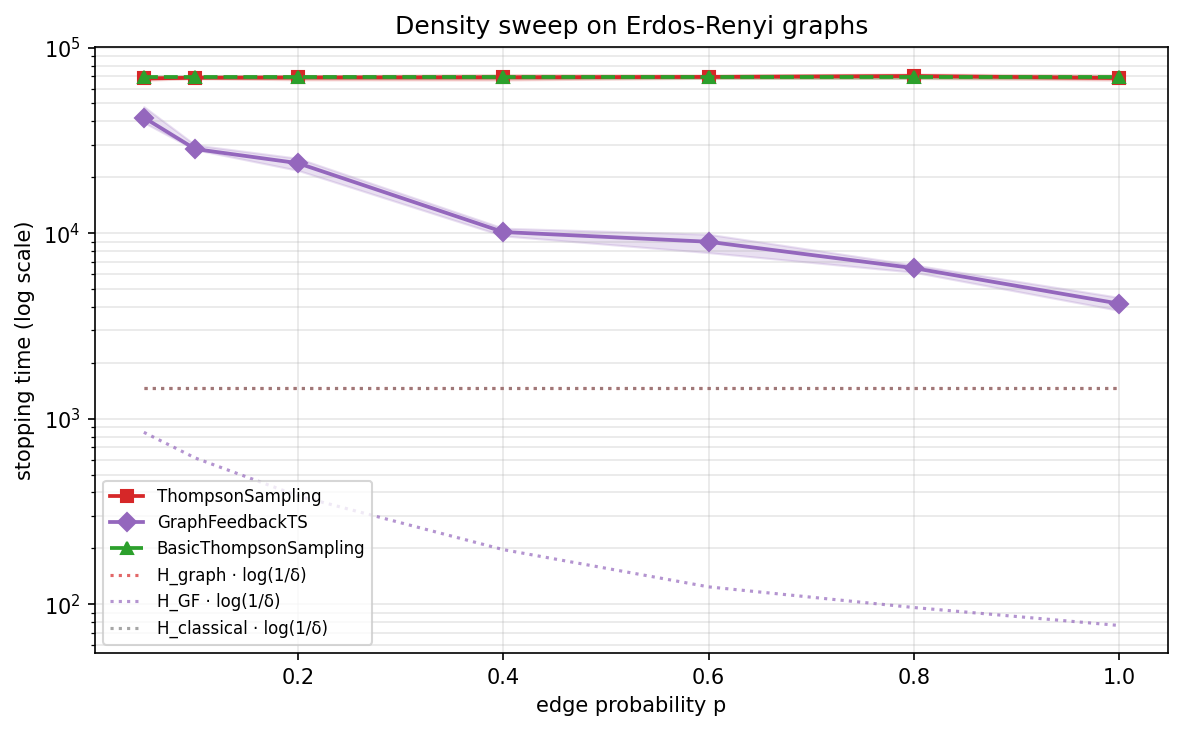
\includegraphics[width=0.75\linewidth]{experiments/outputs/exp2_density_sweep.png}
\caption{\textbf{Graph-feedback density sweep} on Erd\H{o}s--R\'enyi
$n=20$, gap $\Delta=0.3$. Solid lines are median stopping times across 10
seeds with $25$--$75$ percentile shading. Dotted reference lines are the
analytical hardnesses scaled by $\log(1/\delta)$. \texttt{TS-Explore-GF}
tracks $H_{\mathrm{GF}}\log(1/\delta)$ across the entire density range.}
\label{fig:exp-density}
\end{figure}

\begin{table}[t]
\centering
\small
\caption{Hardness measures and median stopping times for the density sweep
($10$ seeds, $\delta=10^{-3}$, $n=20$, $\Delta=0.3$). Both endpoints
match the closed-form values from Corollary~\ref{cor:HGF-bounds}: at
$p=1.0$ (clique) $H_{\mathrm{GF}}=\Delta^{-2}=11.1$, and as $p\to 0$
$H_{\mathrm{GF}}\to (n-1)\Delta^{-2}=211.1$.}
\label{tab:exp-density}
\begin{tabular}{c c c c c c c}
\toprule
$p$ & $H_{\mathrm{GF}}$ & $H_{\mathrm{graph}}$ & $\sum\!\Delta_i^{-2}$
& \texttt{TS-Explore-GF} & \texttt{TS-Explore} & \texttt{Basic TS} \\
\midrule
$0.05$ & $122.2$ & $211.1$ & $211.1$ & $41{,}954$ & $68{,}178$ & $69{,}170$ \\
$0.10$ & $\phantom{0}88.9$ & $211.1$ & $211.1$ & $28{,}386$ & $68{,}786$ & $69{,}170$ \\
$0.20$ & $\phantom{0}55.6$ & $211.1$ & $211.1$ & $23{,}834$ & $69{,}012$ & $69{,}170$ \\
$0.40$ & $\phantom{0}28.5$ & $211.1$ & $211.1$ & $10{,}137$ & $69{,}142$ & $69{,}170$ \\
$0.60$ & $\phantom{0}17.9$ & $211.1$ & $211.1$ & $\phantom{0}8{,}984$ & $69{,}490$ & $69{,}170$ \\
$0.80$ & $\phantom{0}13.9$ & $211.1$ & $211.1$ & $\phantom{0}6{,}476$ & $70{,}284$ & $69{,}170$ \\
$1.00$ & $\phantom{0}11.1$ & $211.1$ & $211.1$ & $\phantom{0}4{,}165$ & $68{,}532$ & $69{,}170$ \\
\bottomrule
\end{tabular}
\end{table}

Three observations support Theorem~\ref{thm:main-fb} and the structural
predictions of Corollary~\ref{cor:HGF-bounds}.
\textbf{(i)} The covering hardness shrinks by an order of magnitude across
the sweep ($H_{\mathrm{GF}}\colon 122.2\to 11.1$) and the median stopping
time of \texttt{TS-Explore-GF} shrinks by the same factor
($41{,}954\to 4{,}165$). The dependence is proportional, as predicted by
$T=O(H_{\mathrm{GF}}\log(1/\delta)+\textnormal{polylog})$.
\textbf{(ii)} At $p=1$ the LP collapses to $\max_i\Delta_i^{-2}=11.1$,
matching the clique closed form $H_{\mathrm{GF}}=\Delta^{-2}$ in
Corollary~\ref{cor:HGF-bounds}. \texttt{TS-Explore-GF} is then $16.4\times$
faster than the graph-smooth \texttt{TS-Explore} ($4{,}165$ vs.\ $68{,}532$)
and $16.6\times$ faster than \texttt{Basic TS} ($4{,}165$ vs.\ $69{,}170$),
confirming the dense-graph gap-collapse predicted by the comparison
paragraph following Theorem~\ref{thm:main-fb}.
\textbf{(iii)} At the sparsest $p=0.05$ the three algorithms collapse to
within $1.65\times$ of each other. This is consistent with the
edge-free closed form $H_{\mathrm{GF}}=(n-1)\Delta^{-2}=211.1$ in
Corollary~\ref{cor:HGF-bounds}: as $p\to 0$ all three hardnesses converge
to the classical $\sum_i\Delta_i^{-2}$.

%-----------------------------------------------------------------------------
\subsection{Smoothness asymptotics under optimal tuning}
\label{sec:exp-asymptotics}
%-----------------------------------------------------------------------------

\paragraph{Setup.}
We use a stochastic block model with five clusters of six arms each, plus
one isolated best arm ($K=31$). Cluster means are
$\{0.9,0.7,0.5,0.3,0.1\}$ and $\mu_{a^\star}=1.0$, so the five gap
magnitudes are $\{0.1,0.3,0.5,0.7,0.9\}$. The classical hardness is
$\sum_{i\neq a^\star}\Delta_{i,c}^{-2}=710.3$ and the asymptotic floor of
Corollary~\ref{cor:eps-limit} is $\max_i\Delta_{i,c}^{-2}=100$. We sweep
the nominal smoothness logarithmically over $\varepsilon\in[10^{-4.5},10^{0}]$
at half-decade resolution (10 points). For each $\varepsilon$ we run
\texttt{TS-Explore} (Algorithm~\ref{algo:ts-explore-graph}) with the
optimally-tuned regularizer $\rho^\star(\varepsilon)=\sigma_0\sqrt{L_1(T)}/\varepsilon$
from~\eqref{eq:rho-star}, where $\sigma_0=2\sigma\sqrt{14}$ and $T$ is
bootstrapped from the classical hardness as
$T=\bigl(\sum_i\Delta_{i,c}^{-2}\bigr)\log(1/\delta)$. As
$\varepsilon$-independent baselines we include \texttt{TS-Explore} with the
fixed default $\rho=1$ and \texttt{Basic TS}. Each cell averages 5 seeds.

\paragraph{Results.}
Figure~\ref{fig:exp-asymptotics} reports three panels: empirical stopping
time (Panel A), analytical $H_\varepsilon$ (Panel B), and competitive-set
size $|\mathcal H_\varepsilon|$ (Panel C). Numerical values are in
Table~\ref{tab:exp-asymptotics}.

\begin{figure}[t]
\centering
\includegraphics[width=0.7\linewidth]{experiments/outputs/exp3_smoothness_asymptotics.png}
\caption{\textbf{Smoothness asymptotics on a $K=31$ SBM.}
Panel A: median stopping time of \texttt{TS-Explore}$(\rho^\star)$ versus
the $\varepsilon$-independent baselines, with $25$--$75$ percentile shading
across 5 seeds. Dotted vertical lines mark the predicted critical
$\varepsilon_i^\star$ values from~\eqref{eq:eps-crit}.
Panel B: analytical $H_\varepsilon$ as defined via
Definition~\ref{def:comp-eps}. Panel C: competitive-set size
$|\mathcal H_\varepsilon|$. Both analytical curves match the staircase
predicted by Definition~\ref{def:comp-eps} and bracket the limits of
Corollary~\ref{cor:eps-limit}.}
\label{fig:exp-asymptotics}
\end{figure}

\begin{table}[t]
\centering
\small
\caption{Smoothness sweep on the $K=31$ SBM, 5 seeds, $\delta=10^{-3}$,
$q=0.1$. The two $\varepsilon$-independent baselines have median
stopping times $1{,}372{,}441$ (\texttt{TS-Explore} with $\rho=1$) and
$1{,}271{,}375$ (\texttt{Basic TS}).}
\label{tab:exp-asymptotics}
\begin{tabular}{c c c c c}
\toprule
$\varepsilon$ & $\rho^\star(\varepsilon)$ & $H_\varepsilon$ &
$|\mathcal H_\varepsilon|$ & \texttt{TS-Explore}$(\rho^\star)$ \\
\midrule
$10^{0}$    & $\phantom{0\,000\,}43.2$       & $710.3$ & $30$ & $1{,}299{,}422$ \\
$10^{-0.5}$ & $\phantom{0\,00\,}136.5$       & $710.3$ & $30$ & $1{,}358{,}820$ \\
$10^{-1}$   & $\phantom{0\,00\,}431.6$       & $710.3$ & $30$ & $1{,}299{,}422$ \\
$10^{-1.5}$ & $\phantom{0\,0}1{,}364.7$      & $710.3$ & $30$ & $1{,}185{,}749$ \\
$10^{-2}$   & $\phantom{0\,0}4{,}315.6$      & $710.3$ & $30$ & $\phantom{0,}557{,}498$ \\
$10^{-2.5}$ & $\phantom{0\,}13{,}647.0$      & $704.1$ & $24$ & $\phantom{0,}\mathbf{265{,}361}$ \\
$10^{-3}$   & $\phantom{0\,}43{,}155.7$      & $670.7$ & $12$ & $\phantom{0,}268{,}100$ \\
$10^{-3.5}$ & $\phantom{0}136{,}470.2$       & $611.1$ & $\phantom{0}6$ & $\phantom{0,}362{,}375$ \\
$10^{-4}$   & $\phantom{0}431{,}556.7$       & $611.1$ & $\phantom{0}6$ & $\phantom{0,}634{,}435$ \\
$10^{-4.5}$ & $1{,}364{,}702.1$              & $100.0$ & $\phantom{0}0$ & $1{,}225{,}829$ \\
\bottomrule
\end{tabular}
\end{table}

The structural predictions of Corollary~\ref{cor:eps-limit} (i)--(ii) match
the data exactly: as $\varepsilon$ decreases past the corresponding
$\varepsilon_i^\star$ thresholds, $|\mathcal H_\varepsilon|$ shrinks
$30\to 24\to 12\to 6\to 0$, and $H_\varepsilon$ correspondingly descends
the staircase $710\to 100$, hitting the asymptotic floor
$\max_i\Delta_{i,c}^{-2}=100$ exactly at the $\varepsilon$ where the last
arm exits the competitive set.

The empirical stopping time achieves a $5.12\times$ speedup of the
optimally-tuned \texttt{TS-Explore} over its $\rho=1$ counterpart at the
empirical optimum $\varepsilon^\dagger\approx 10^{-2.5}$
(median $265{,}361$ vs.\ $1{,}372{,}441$), and a $4.79\times$ speedup over
\texttt{Basic TS} ($265{,}361$ vs.\ $1{,}271{,}375$). This validates the
rho-tuning gain claimed by Theorem~\ref{thm:main-mis}.

\paragraph{Remark on the empirical optimum.}
Panel A is non-monotone in $\varepsilon$: the stopping time drops by a
factor of five from $\varepsilon=10^0$ to $\varepsilon^\dagger\approx
10^{-2.5}$, then climbs back to baseline as $\varepsilon$ shrinks further.
This is consistent with Theorem~\ref{thm:main-mis} read as an upper bound:
the dominant prefactor in Lemma~\ref{lem:terminate-graph} is
$186\,C(t)\,L(t)/\Delta_{i,c}^2$, which is increasing in $\rho^\star$ and
hence decreasing in $\varepsilon$. For sufficiently small $\varepsilon$
this prefactor dominates the $H_\varepsilon$ reduction, so the bound's
predicted decrease becomes loose. Algorithmically, the Thompson samples
in line~12 of Algorithm~\ref{algo:ts-explore-graph} are drawn from
$\mathcal{N}\!\bigl(\widehat\mu_i, C(\delta,q,t)/t_{\mathrm{eff},i}\bigr)$
with no explicit bias correction, while the regularised estimator
$\widehat{\bm\mu}$ carries a bias of order $\rho\varepsilon/\sqrt{t_{\mathrm{eff},i}}
=\sigma_0\sqrt{L_1(T)}/\sqrt{t_{\mathrm{eff},i}}$ under~\eqref{eq:rho-star}.
This bias persists at the same order as the sampling standard deviation
throughout the sweep, so as $\rho^\star\to\infty$ the all-samples-agree
stopping rule loses leverage. The empirical optimum $\varepsilon^\dagger$
is therefore a practical recommendation: tune $\varepsilon$ to where the
staircase has dropped $H_\varepsilon$ by a constant factor relative to
$\sum_i\Delta_{i,c}^{-2}$, not to the asymptotic floor.

%=============================================================================
